% VUT FIT MITAI
% MSZ 2021/2022
% Author: Vladimir Dusek
% Login: xdusek27

%%%%%%%%%%%%%%%%%%%%%%%%%%%%%%%%%%%%%%%%%%%%%%%%%%%%%%%%%%%%%%%%%%%%%%%%%%%%%%%%

% Path to figures
\graphicspath{{avs/architektura_superskalarnich_procesoru/figures}}

%%%%%%%%%%%%%%%%%%%%%%%%%%%%%%%%%%%%%%%%%%%%%%%%%%%%%%%%%%%%%%%%%%%%%%%%%%%%%%%%

\chapter{AVS~--~Architektura superskalárních procesorů a algoritmy zpracování instrukcí mimo pořadí, predikce skoků.}

%%%%%%%%%%%%%%%%%%%%%%%%%%%%%%%%%%%%%%%%%%%%%%%%%%%%%%%%%%%%%%%%%%%%%%%%%%%%%%%%

\section{Zdroje}

\begin{compactitem}
    \item \path{AVS_2019-09-23.mp4}
    \item \path{AVS_2019-09-30.mp4}
    \item \path{AVS_2019-10-07.mp4}
    \item \path{AVS_2019-10-14.mp4}
    \item \path{AVS-01.pdf}
    \item \path{AVS-02.pdf}
    \item \path{AVS-03.pdf}
    \item \path{AVS-04.pdf}
\end{compactitem}

%%%%%%%%%%%%%%%%%%%%%%%%%%%%%%%%%%%%%%%%%%%%%%%%%%%%%%%%%%%%%%%%%%%%%%%%%%%%%%%%

\section{Úvod a kontext}

\begin{compactitem}
    \item Chceme zvyšovat výpočetní výkon. Jak na to? \begin{compactitem}
        \item Zvyšovat počet tranzistorů, tam brzy narazíme na fyzikální limity.
        \item Počítat efektivněji (bez čekání) a paralelizovat.
    \end{compactitem}

    \item \textbf{Moorův zákon} \begin{compactitem}
        \item Počet tranzistorů na čipu se zdvojnásobuje každé dva roky při zachování stejné ceny.
        \item Se snižováním rozměrů tranzistorů se rychlost zvyšuje, příkon snižuje.
        \item Nejedná se o fyzikální zákon, spíše jde o empirický vztah vypozorovaný z historických dat.
    \end{compactitem}

    \item \textbf{Úrovně paralelismu} \begin{compactitem}
        \item Paralelní provádění instrukcí (ILP, \textit{instruction level parallelism}).
        \item Střídání vláken na CPU (TLP, \textit{thread level parallelism}).
        \item Paralelní zpracování dat (DLP, \textit{data level parallelism}).
        \item Rozdělení úloh na vlákna/procesy na více jader.
    \end{compactitem}

    \item \textbf{Amdahlův zákon} \begin{compactitem}
        \item Vyjadřuje kdy mý smysl něco optimalizovat (zrychlovat) a kdy ne, tj. které části má smysl paralelizovat.

        $$ \lim_{P \rightarrow \infty}{S(P)} = \frac{1}{\alpha} $$
        \item kde \begin{compactitem}
            \item $P$ je počet procesorů;
            \item $S(P)$ funkce dosáhnutého zrychlení v závislosti na $P$;
            \item $\alpha$ sekvenční část úlohy (ze své podstaty).
        \end{compactitem}

        \item Myšlenka: Pro nekonečný počet procesorů bude maximální možné zrychlení převrácená hodnota poměru z principu sekvenční části ku paralilizovatelné.

        \item Kdy má smysl paralelizovat? Když z principu sekvenční část je malá.

        \begin{figure}[H]
            \centering
            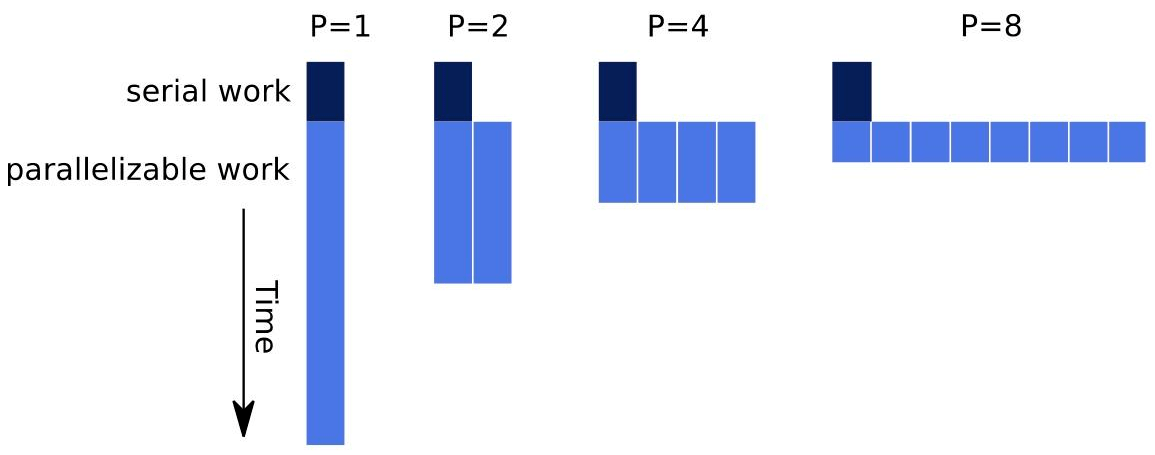
\includegraphics[width=1\linewidth]{amdahl.png}
            \caption{Amdahlův zákon.}
        \end{figure}
    \end{compactitem}

\end{compactitem}

%%%%%%%%%%%%%%%%%%%%%%%%%%%%%%%%%%%%%%%%%%%%%%%%%%%%%%%%%%%%%%%%%%%%%%%%%%%%%%%%

\section{Vývoj procesorů}

\begin{compactitem}
    \item Metriky: \begin{compactitem}
        \item CPI (\textit{clocks per instruction}) -- Kolik taktů trvá jedna instrukce v průměru.

        \item IPC (\textit{instructions per clock}) -- Kolik instrukcí se vykoná za jeden takt v průměru.
        $$ \text{IPC} = \frac{1}{\text{CPI}} $$

        \item R, IPS (\textit{instructions per second}) -- Výkon; kolik instrukcí se vykoná za sekundu.

        \item f [Hz] -- Frekvence; počet taktů procesoru za sekundu.
    \end{compactitem}
\end{compactitem}

\subsection{Subskalární procesor}

\begin{compactitem}
    \item Sekvenční zpracování instrukcí (Von Neumannova technika).
    \item Každá instrukce může trvat jiný počet taktů.

    \item Příklad:
    \begin{figure}[H]
        \centering
        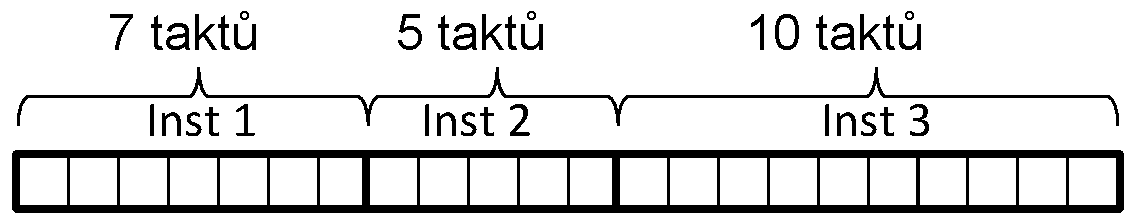
\includegraphics[width=0.75\linewidth]{subscalar.pdf}
        \caption{Vykonávání instrukcí subskalárním procesorem; 3 instrukce, 22 taktů.}
    \end{figure}

    \begin{compactitem}
        \item CPI, IPC:
        $$ \text{CPI} = \frac{22}{3} \approx 7,33 $$
        $$ \text{IPC} \approx \frac{1}{7,33} \approx 0,14 $$
        \item IPS při frekvenci 5 GHz:
        $$ \text{IPS} = 5 \times 10^9 \times \frac{3}{22} \approx 682 \times 10^6 $$
    \end{compactitem}
\end{compactitem}

\subsection{Skalární procesor}

\begin{compactitem}
    \item Řetězená linka (\uv{pipeline}).
    \item Všechny instrukce musí trvat stejný počet taktů.
    \item Cíl: jedna instrukce každý takt (v limitě $N \rightarrow \infty$), reálně je to horší, kvůli tzv. pokutám (viz dále).

    \item Příklad:
    \begin{figure}[H]
        \centering
        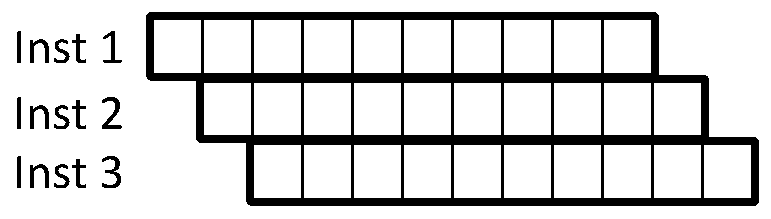
\includegraphics[width=0.5\linewidth]{scalar.pdf}
        \caption{Vykonávání instrukcí skalárním procesorem; 3 instrukce každá trvá 10 taktů.}
    \end{figure}

    \begin{compactitem}
        \item CPI, IPC:
        $$ \text{CPI} = \frac{10 + 3 - 1}{3} = 4 $$
        $$ \text{IPC} = \frac{1}{4} = 0,25 $$
        \item IPS při frekvenci 5 GHz:
        $$ \text{IPS} = 5 \times 10^9 \times 0,25 \approx 1250 \times 10^6 $$
    \end{compactitem}
\end{compactitem}

\subsection{Superskalární procesor}

\begin{compactitem}
    \item Superřetězená linka -- několik řetězených linek.
    \item Možnost vykonávat několik instrukcí za takt.
    \item Jak to funguje? \begin{compactitem}
        \item Mějme $N$ linek (dnes běžné 6-9) a příslušné dekodéry instrukcí.
        \item Dekodéry vybírají instrukce z linek tak, aby je bylo možné nezávisle zpracovat.
        \item Dokáží vydávat až $N$ instrukcí za takt.
    \end{compactitem}
    \item Platí:
    $$ \text{IPC} < N $$
    \item Využívá přeskládání pořadí instrukcí tak, jak procesoru vyhovuje, ale nemění sémantiku programu.
\end{compactitem}

%%%%%%%%%%%%%%%%%%%%%%%%%%%%%%%%%%%%%%%%%%%%%%%%%%%%%%%%%%%%%%%%%%%%%%%%%%%%%%%%

\section{Architektura skalárních procesorů}

\begin{compactitem}
    \item Jak se realizuje? \begin{compactitem}
        \item Programová logika je rozdělena na části a mezi ně jsou vloženy oddělovací registry.
    \end{compactitem}

    \begin{figure}[H]
        \centering
        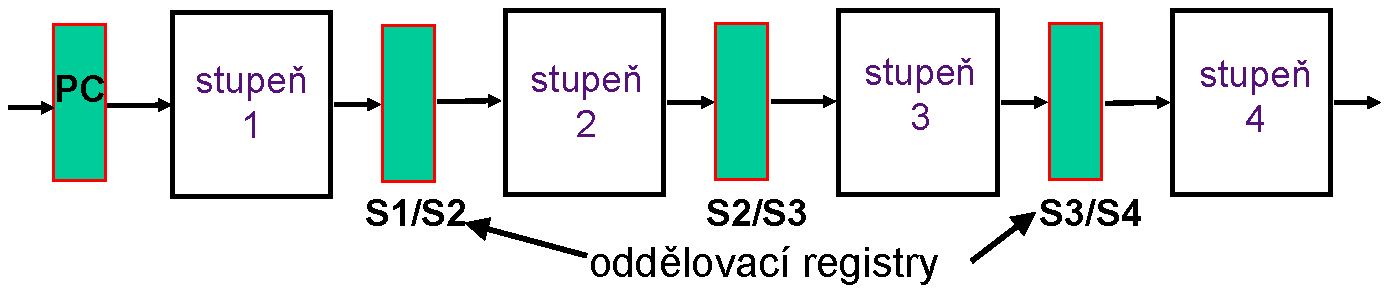
\includegraphics[width=1\linewidth]{idealni_retezena_linka.pdf}
        \caption{Ideální řetězená linka.}
    \end{figure}

    \item Jaké jsou předpoklady pro zřetězené zpracování? \begin{compactitem}
        \item Nepřetržitý přísun dat.
        \item Instrukce musí být možná rozdělit na sekvenci nezávislých kroků.
        \item Trvání kroků by mělo být přibližně stejné.
    \end{compactitem}

    \item Co má vliv na celkové dosažitelné zrychlení? \begin{compactitem}
        \item Přestávky a pokuty způsobené zpracováním závislostí (např. před sčítáním musím načíst data z paměti).
        \item Náběh a doběh (\uv{naplnění} a \uv{vypláchnutí} linky).
        \item Zpoždění oddělovacích registrů.
    \end{compactitem}

    \item Zrychlení skalární linky oproti subskalární. \begin{compactitem}
        \item Každá instrukce probíhá v několika krocích, tzv. mikroinstrukcích.

        \item Výkonnost ($R$):
        $$ R = \text{IPS} = \frac{\text{počet instrukcí}}{\text{čas}} $$

        \item Zrychlení linky pro $N$ instrukcí ($S_N$):
        $$ S_N = \frac{\text{skalární výkon}}{\text{subskalární výkon}} = \frac{\text{subskalární čas}}{\text{skalární čas}} $$

        \item Potom:
        $$ \text{subskalární čas} = N \times t_i = N \times \tau \times k $$
        $$ \text{skalární čas} = (N - 1 + k) \times (\tau + t_d) $$
        \begin{compactitem}
            \item $N$ je počet instrukcí;
            \item $t_i$ je průměrná doba trvání instrukce;
            \item $k$ je počet mikroinstrukcí (počet stupňů);
            \item $\tau$ je doba trvání mikroinstrukce;
            \item $t_d$ je doba zpoždění registru.
        \end{compactitem}
    \end{compactitem}

    \item Zrychlení při pozastavování linky. \begin{compactitem}
        \item V realitě se maximálnímu dosažitelnému zrychlení budeme chtít pouze přiblížit, jsou případy, kdy je nutné linky zastavit (různé kolize, viz dále).
        \item Dobu zastavování linky můžeme zprůměrovat na pokutu $q$ taktů vztaženou na každou instrukci.
        \item Počet taktů na 1 instrukci je pak $\text{CPI} = 1+q$.
        $$ \text{skalární čas} = (N - 1 + k) \times (\tau + t_d) \times (1 + q) $$

        \item Zpomalení registrů často nemusíme řešit -- je příliš malé, proto lze zanedbat.
    \end{compactitem}

\end{compactitem}

%%%%%%%%%%%%%%%%%%%%%%%%%%%%%%%%%%%%%%%%%%%%%%%%%%%%%%%%%%%%%%%%%%%%%%%%%%%%%%%%

\section{Architektura skalárních procesorů RISC}

\begin{compactitem}
    \item RISC (\textit{reduced instruction set computer}) -- Redukovaná (minimální) instrukční sada.

    \item CISC (\textit{complex instruction set computing}) -- Komplexní instrukční sada.

    \item Dnešní moderní procesory jsou CISC, ale \uv{jádro} mají RISC.

    \item CISC funguje pouze jako nadstavba ve fázi decode, kdy je CISC instrukce dekódována na několik RISC instrukcí.

    \item RISC má velké množství registrů, v jednom taktu umí číst i zapisovat (brány zápisu, brány čtení).

    \begin{figure}[H]
        \centering
        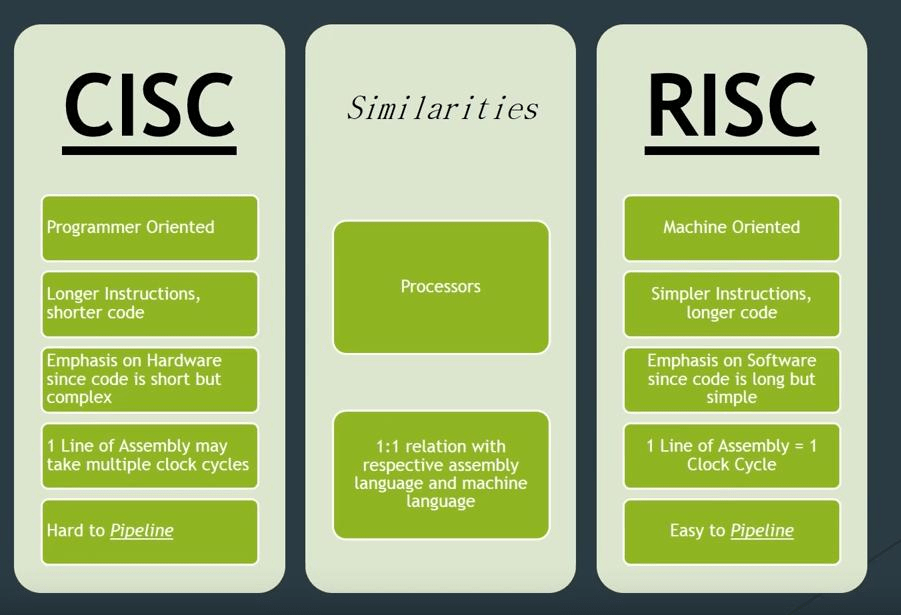
\includegraphics[width=1\linewidth]{cisc_vs_risc.png}
        \caption{CISC vs RISC.}
    \end{figure}

    \item Charakteristika RISC instrukcí: \begin{compactitem}
        \item Všechny instrukce mají stejnou velikost (32/64 bitů).
        \item Málo formátů instrukcí a formáty jsou pravidelné.
        \item Přístup do paměti mají pouze instrukce LOAD a STORE.
        \item Hodně registrů.
    \end{compactitem}

    \item Formáty instrukcí: \begin{compactitem}
        \item Register type: \path{op} \path{src1} \path{src2} \path{dst} (např. sčítání, odčítání).

        \item Imm type: \path{op} \path{src/dst}  \path{address} (např. načítání, ukládání).

        \item Jump type: \path{target_address} (např. skok).
    \end{compactitem}

    \item Stupně řetězeného zpracování: \begin{compactitem}
        \item IF (\textit{instruction fetch}) -- Načtení instrukce z instrukční cache na základě hodnoty v PC registru.

        \item ID (\textit{instruction decode}) -- Dekódování instrukce, získání opcode, získání dat z registrů do procesoru.

        \item EX (\textit{execute}) -- Počítání, ADD sčítá, LOAD/STORE počítá adresu, JUMP počítá podmínku.

        \item MA (\textit{memory access}) -- ADD nic, LOAD čte z datové cache, STORE zapisuje do datové cache, JUMP zapisuje do PC registru.

        \item WB (\textit{write back}) -- ADD zapisuje výsledek do registru DST, LOAD zapisuje do registru, STORE nedělá nic.
    \end{compactitem}

    \begin{figure}[H]
        \centering
        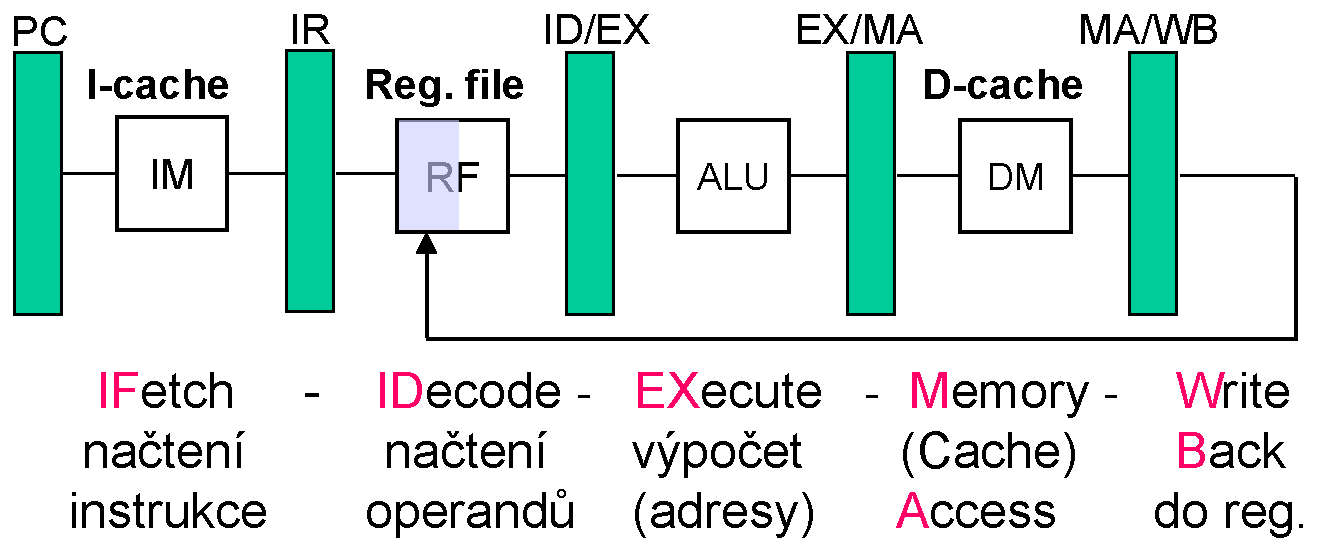
\includegraphics[width=1\linewidth]{risc_stupne_retezeneho_zpracovani.pdf}
        \caption{Stupně řetězeného zpracování RISC. Zeleně jsou oddělovací registry, dále instrukční cache, registrové pole, ALU, datová cache.}
    \end{figure}

    \begin{figure}[H]
        \centering
        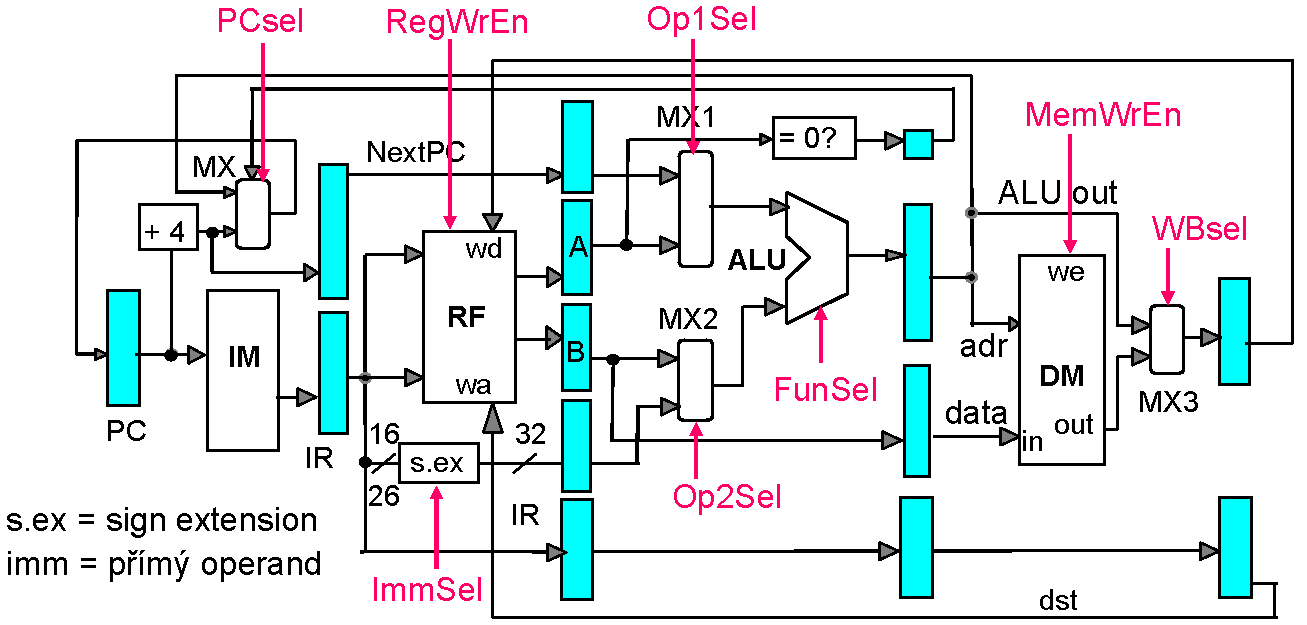
\includegraphics[width=1\linewidth]{risc_pipeline.pdf}
        \caption{Klasická RISC pipeline (fáze IF, ID, EX, MA, WB). To co se při fázi WB zapíše do registrového pole lze hned v tom samém taktu použít!}
    \end{figure}
\end{compactitem}

%%%%%%%%%%%%%%%%%%%%%%%%%%%%%%%%%%%%%%%%%%%%%%%%%%%%%%%%%%%%%%%%%%%%%%%%%%%%%%%%

\section{Architektura superskalárních procesorů}

\begin{compactitem}
    \item Jak zrychlit dobu výpočtu programu?
    $$ \text{doba výpočtu} = IC \times CPI \times T $$
    \begin{compactitem}
        \item IC (\textit{instruction count}) -- Počet provedených instrukcí. Jak snížit? \begin{compactitem}
            \item Optimalizací kódu, napsat program líp.
        \end{compactitem}

        \item CPI -- Počet taktů na instrukci. Jak snížit? \begin{compactitem}
            \item Více instrukcí v jednom stupni -- $m$-cestný superskalární procesor.
            \item Reálně dosažitelná hodnota IPC (kolik instrukcí končí v taktu) je vždy značně nižší než $m$.
        \end{compactitem}

        \item T -- doba vykonání jednoho taktu. Jak snížit? \begin{compactitem}
            \item Větší počet stupňů linky (až 30).
            \item S tím jsou spojené velké pokuty, vyšší příkon, doba zpoždění registrů.
        \end{compactitem}
    \end{compactitem}
\end{compactitem}

\subsection{Fáze superskalárního zpracování}

\begin{compactitem}
    \item \textbf{Front end} -- IF, ID. \begin{compactitem}
        \item Načítá a dekóduje několik instrukcí najednou, počet se mění dynamicky.
        \item $M$-cestný superskalár znamená, že vydává až $m$ instrukcí do funkčních jednotek v 1 taktu.
    \end{compactitem}

    \item \textbf{Back end} -- EX, MA, WB. \begin{compactitem}
        \item Provádí a ukládá výsledky několika instrukcí souběžně.
        \item Některé stupně jsou rozděleny na podstupně.
    \end{compactitem}
\end{compactitem}

\subsection{Dělení superskalárních procesorů}

\begin{compactitem}
    \item Dle způsobu jakým instrukce opouštějí front-end.
\end{compactitem}

\begin{compactitem}
    \item \textbf{INO -- in-order} \begin{compactitem}
        \item Instrukce jsou vykonávány podle pořadí v programu, po vyřešení konfliktů.
        \item Jednotlivé stupně mohou mít různé zpoždění nebo propustnost instrukcí za takt.
        \item Front end opouští až $m$ instrukcí v jednom taktu.
    \end{compactitem}

    \begin{figure}[H]
        \centering
        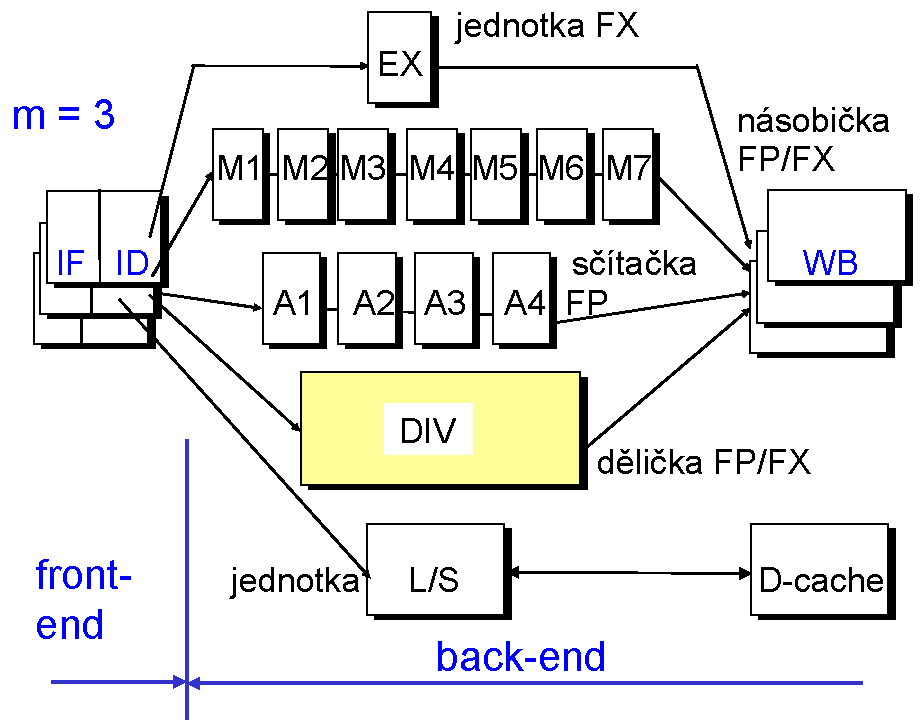
\includegraphics[width=0.75\linewidth]{ino.pdf}
        \caption{Příklad skalárního in-order procesoru.}
    \end{figure}

    \item \textbf{OOO -- out-of-order} \begin{compactitem}
        \item Mohou vykonávat instrukce mimo pořadí v programu, nepravé konflikty vyřešeny přejmenováním v HW, RAW řešeny čekáním rozpracovaných instrukcí.
        \item Back end -- Vykonává se out-of-order.
        \item Front end -- Vykonává se in-order (jinak by to pochopitelně byl nesmysl).
        \item První prediktor skoku se nechází už ve fázi IF.
        \item Reorder Buffer (ROB) -- Seřazovací paměť.
        \item Rename Register Field (RRF) -- Registry pro přejmenování.
        \item Dispatch (DI) -- Nová fáze instrukce pro rozeslání instrukcí do rezervačních stanic a ROB.
    \end{compactitem}

    \begin{figure}[H]
        \centering
        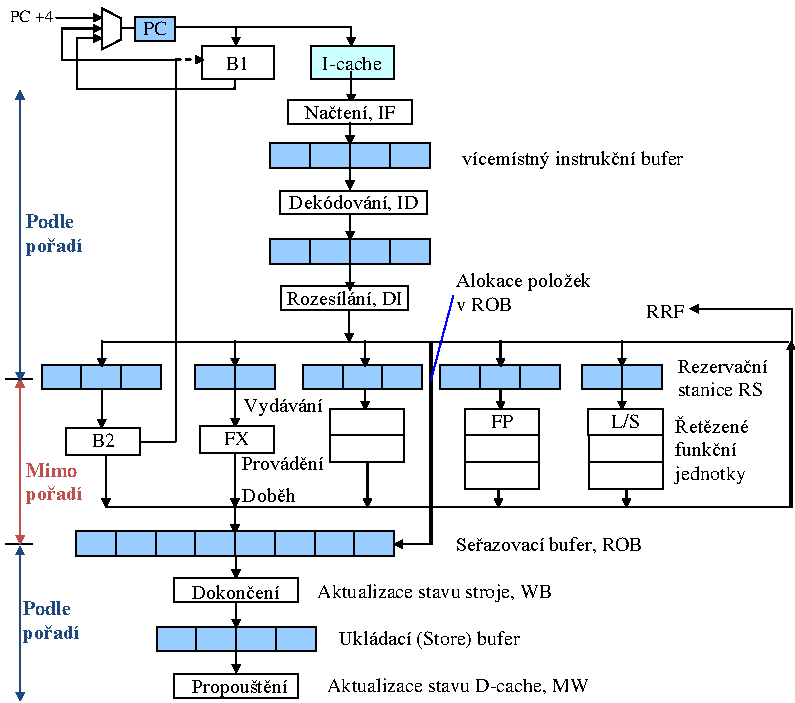
\includegraphics[width=1\linewidth]{ooo.pdf}
        \caption{Generická OOO superskalární architektura. Po dekódování se instrukce mohou zpracovat v libovolném pořadí, ale na konci se musí opět seřadit.}
    \end{figure}
\end{compactitem}

\subsection{Rysy superskalárních procesorů}

\begin{compactitem}
    \item Paralelní řetězené linky (INO i OOO). \begin{compactitem}
        \item Časový i prostorový paralelismus (paralelní načítání, dekódování, vydávání instrukcí do FJ, jejich paralelní provádění a dokončování).
    \end{compactitem}

    \item Přejmenování registrů v HW (OOO). \begin{compactitem}
        \item Odstraní konflikty WAR a WAW (viz dále).
    \end{compactitem}

    \item Dynamické plánování instrukcí out-of-order (OOO). \begin{compactitem}
        \item Po dekódování čekají instrukce na své operandy, které se tvoří. Jakmile jsou operandy připraveny, spustí se operace.
        \item Instrukce, včetně přístupů do paměti, jsou zpracovávány v jiném pořadí oproti pořadí v programu (OOO).
    \end{compactitem}

    \item Seřazovací paměť (OOO). \begin{compactitem}
        \item Stupeň WB pomocí ní zajišťuje ukládání výsledků v pořadí určeném zdrojovým kódem.
    \end{compactitem}

    \item Spekulativní zpracování instrukcí (OOO). \begin{compactitem}
        \item Spekulace, že skok dopadne podle predikce nebo že dopředu načtená data se již nezmění.
    \end{compactitem}
\end{compactitem}

%%%%%%%%%%%%%%%%%%%%%%%%%%%%%%%%%%%%%%%%%%%%%%%%%%%%%%%%%%%%%%%%%%%%%%%%%%%%%%%%

\section{Konflikty při řetězeném zpracování instrukcí}

\begin{compactitem}
    \item Instrukce může záviset na něčem co produkuje dřívější instrukce. \begin{compactitem}
        \item Datová závislost -- závislost se může týkat hodnot dat.
        \item Řídící závislost -- závislost se může týkat adresy příští instrukce.
    \end{compactitem}

    \item Instrukce v řetězené lince může potřebovat prostředek, který právě používá jiná instrukce. \begin{compactitem}
        \item Strukturní závislost.
    \end{compactitem}

    \item Jak konflikty řešíme? \begin{compactitem}
        \item Přejmování registrů.
        \item Vyplněný prázdných taktů užitečnými instrukcemi.
        \item Přehození pořadí instrukcí bez změny sémantiky programu s hlídáním zpoždění mezi operacemi.
        \item Rozbalení smyček.
        \item SW řetězení smyček v programu, případně v kombinaci s rozbalením.
        \item Překladač zná kolik má jaká instrukce zpoždění.
    \end{compactitem}
\end{compactitem}

\subsection{Datová závislost}

\begin{compactitem}
    \item Dále dělíme na: \begin{compactitem}
        \item \textbf{Pravé} (\textit{true dependencies}) -- Nejde s nimi \uv{nic moc dělat}, definují sémantiku programu.
        \item \textbf{Nepravé} (\textit{false dependencies}) -- Mohou vzniknout pouze u superskalárních procesorů při vykonávání instrukcí mimo pořadí v programu.
    \end{compactitem}
\end{compactitem}

\subsubsection{RAW (\textit{read after write})}
\begin{compactitem}
    \item Pravý konflikt.

    \item Instrukce $I_2$ pracuje s výsledkem instrukce $I_1$, který ještě nebyl vypočítán nebo načten. I když je instrukce $I_2$ provedena po instrukci $I_1$, tak $I_1$ instrukce byla zpracována pouze částečně v rámci pipeline.

    \item Řešení: Nová datová cesta (zkratka), tzv. \textbf{bypass}. Např. můžeme dostat data z výstupu ALU na vstup ALU v dalším taktu.

    \begin{figure}[H]
        \centering
        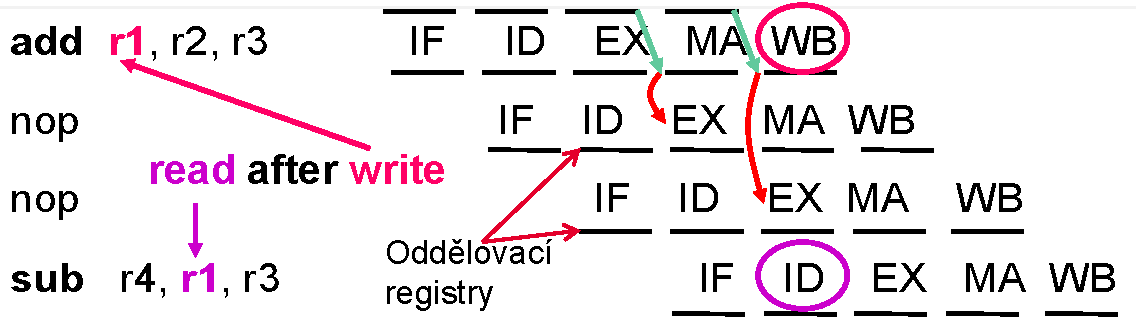
\includegraphics[width=0.8\linewidth]{raw_1.pdf}
        \caption{Příklad RAW (nop značí čekání), instrukce sub čte výsledek zapsaný instrukcí add. Lze řešit bypassem.}
    \end{figure}

    \begin{figure}[H]
        \centering
        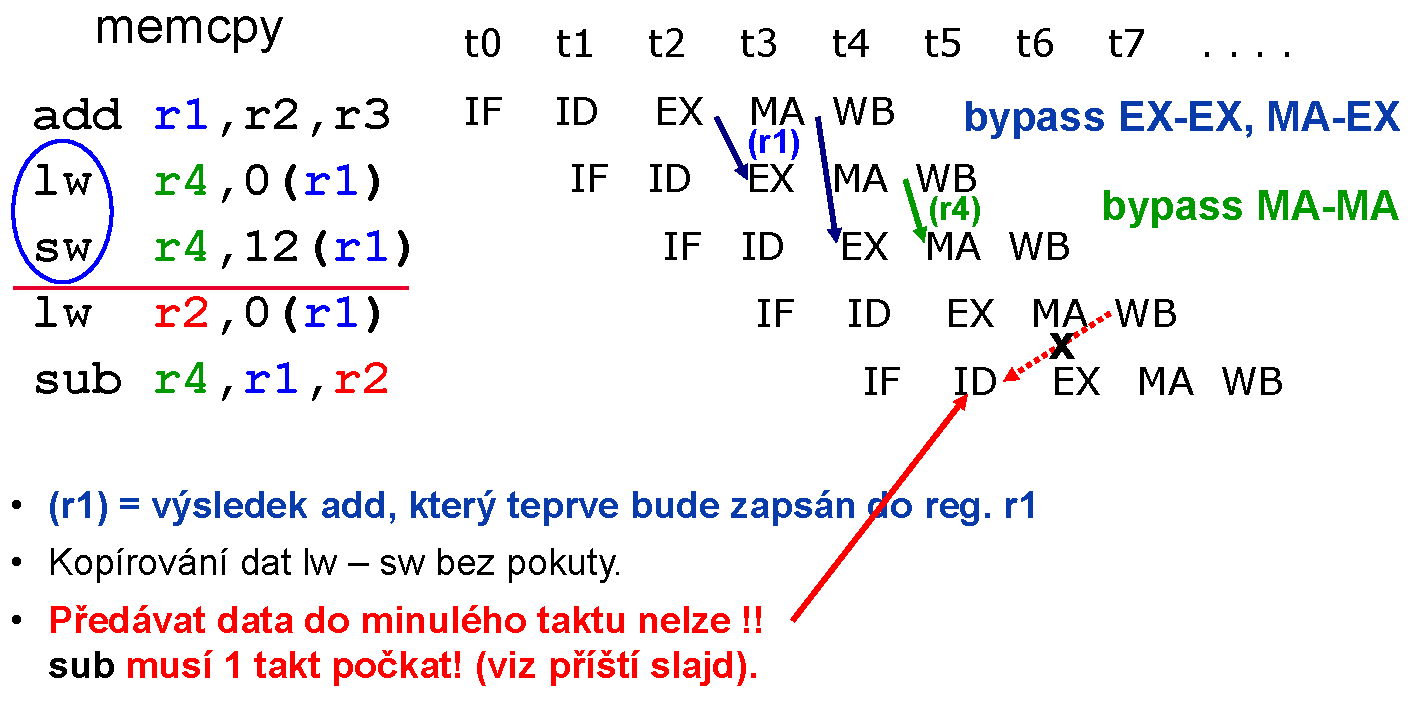
\includegraphics[width=0.95\linewidth]{raw_2.pdf}
        \caption{Příklad RAW, instrukce sub čte výsledek zapsaný instrukcí lw. Nelze (kompletně) řešit bypassem, stále bude nutné čekat.}
    \end{figure}
\end{compactitem}

\subsubsection{WAR (\textit{write after read})}
\begin{compactitem}
    \item Nepravý konflikt.
    \item Přepsání dat, která ještě někdo měl číst.

    \begin{figure}[H]
        \centering
        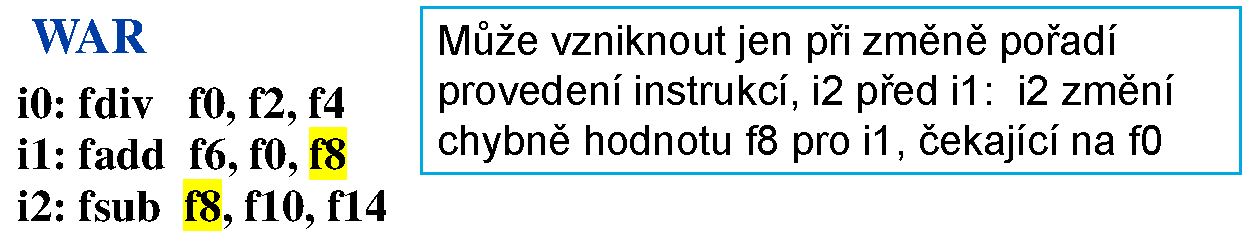
\includegraphics[width=0.8\linewidth]{war.pdf}
        \caption{Příklad WAR.}
    \end{figure}
\end{compactitem}

\subsubsection{WAW (\textit{write after write})}
\begin{compactitem}
    \item Nepravý konflikt.
    \item Instrukce, která byla naplánována později se přesune dopředu a přepíše hodnotu registru, kterou chtěla zapsat nějaká jiná instrukce.

    \begin{figure}[H]
        \centering
        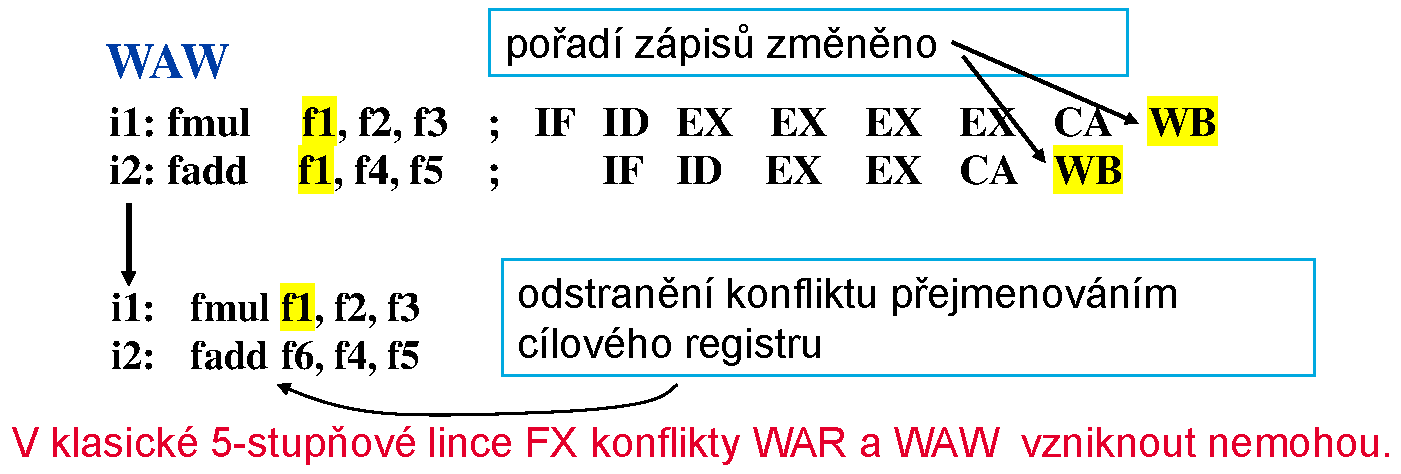
\includegraphics[width=0.8\linewidth]{waw.pdf}
        \caption{Příklad WAW.}
    \end{figure}
\end{compactitem}

\subsection{Řídící závislost}

\begin{compactitem}
    \item Týká se podmíněných/nepodmíněných skoků.
    \item Ve fázi EX se počítá jestli a kam skočit.
    \begin{figure}[H]
        \centering
        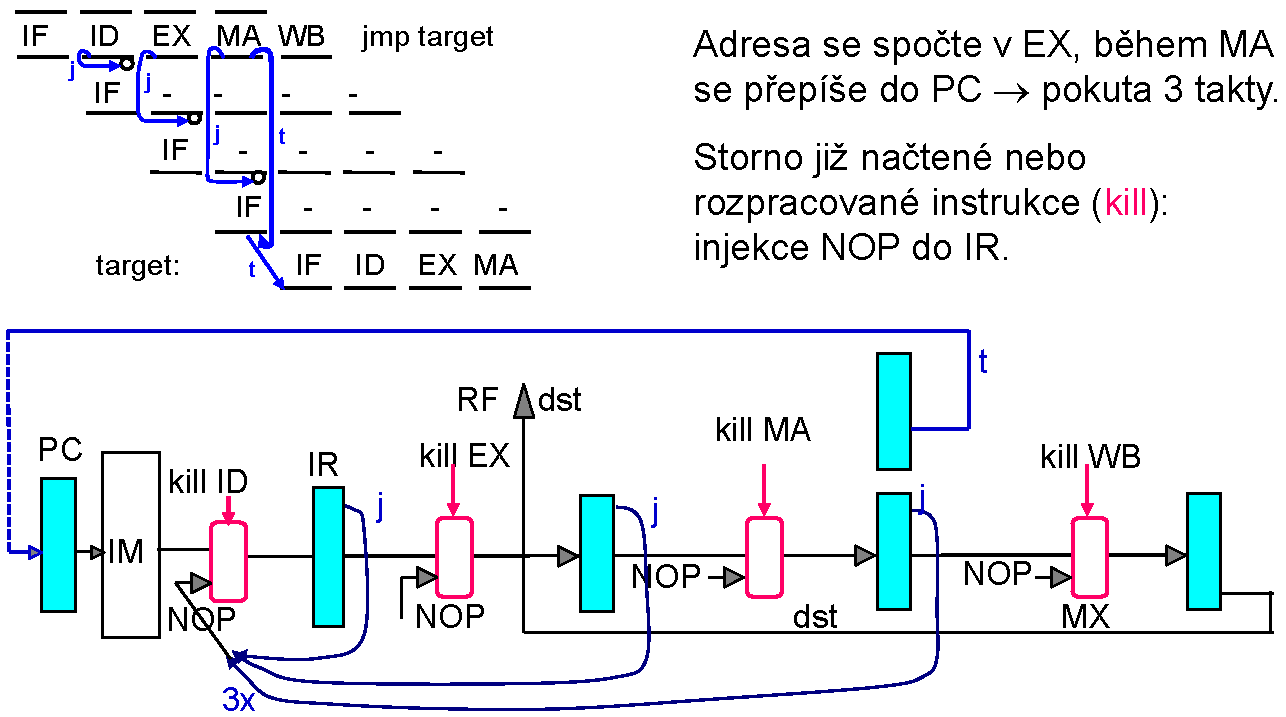
\includegraphics[width=1\linewidth]{ridici_konflikt.pdf}
        \caption{Řídící konflikt.}
    \end{figure}

    \item Co dělat abychom nemuseli čekat 3 takty na zjištění adresy další instrukce při skoku? \begin{compactitem}
        \item Pro \textbf{nepodmíněný skok} přidáme další hardware (sčítačku) ve stupni ID, zjistíme, že se jedná o skok a ihned můžeme připočíst / odečíst offset a víme odkud brát další instrukci. Výsledná pokuta bude 1 takt.
        \begin{figure}[H]
            \centering
            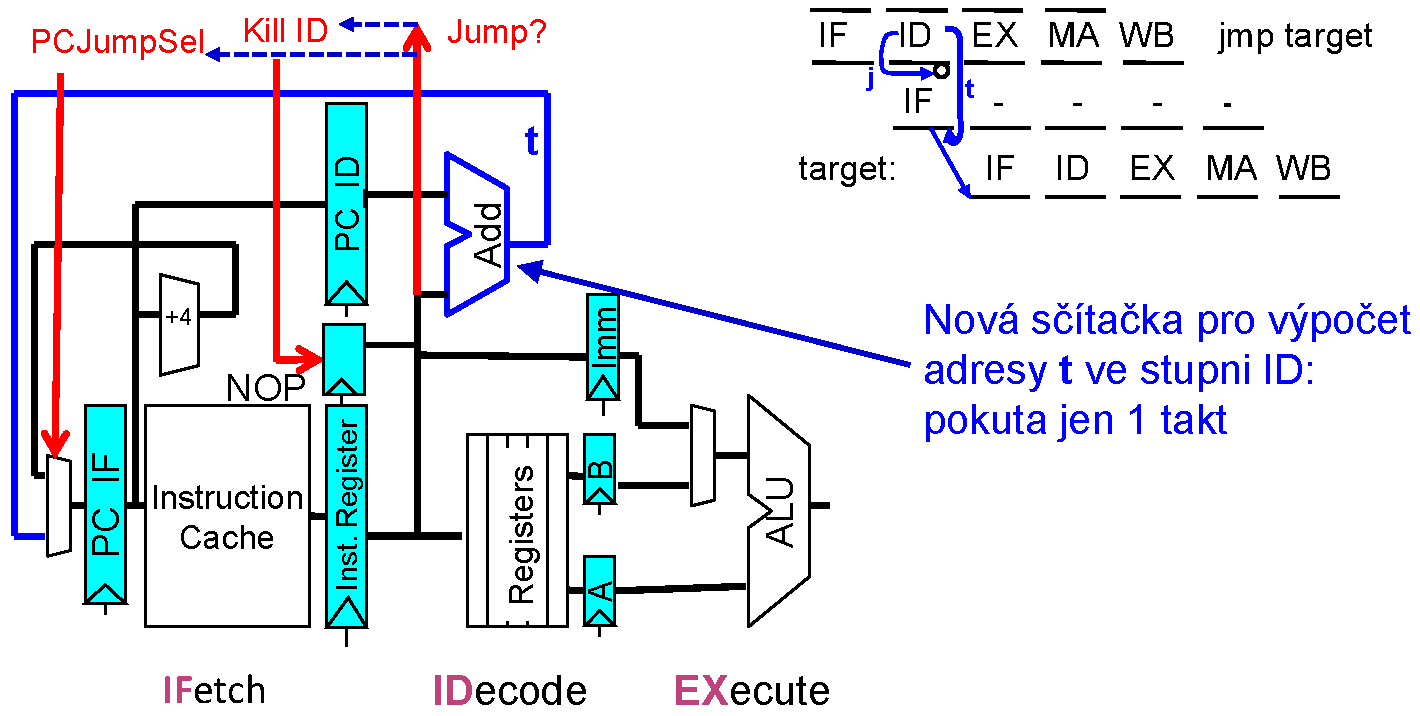
\includegraphics[width=1\linewidth]{reseni_skok.pdf}
            \caption{Úprava HW pro nepodmíněné skoky (jump).}
        \end{figure}

        \item Pro \textbf{podmíněný skok} přidáme také další hardware (sčítačku, komparátor pro test na nulu) ve stupni ID. Pokud skočím, je pokuta 1 takt, pokud ne, žádný.
        \begin{figure}[H]
            \centering
            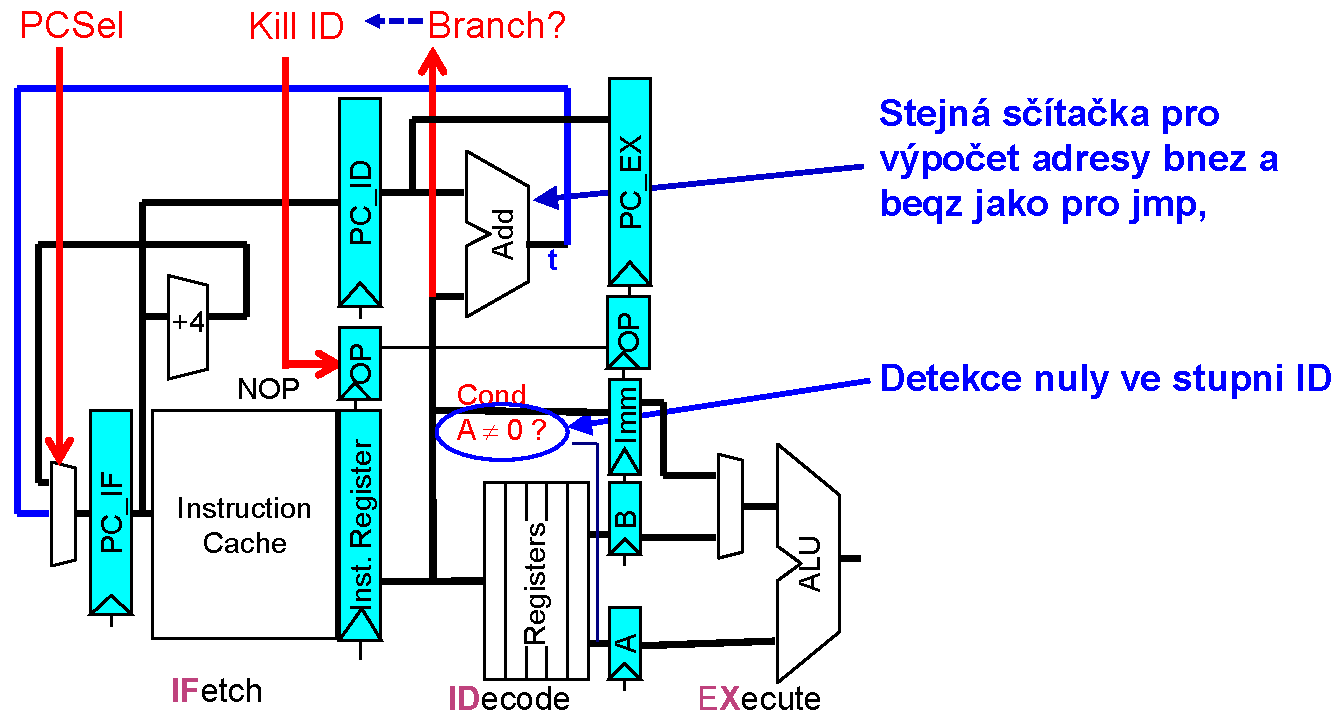
\includegraphics[width=1\linewidth]{reseni_podmineny_skok.pdf}
            \caption{Úprava HW pro podmíněné skoky (bnez, beqz).}
        \end{figure}

        \item U složitějších podmínek můžu vyhodnotit až po EX fázi, nutně tedy pokuta 1 takt vždy, pokud skočím tak 2 takty.
    \end{compactitem}

\end{compactitem}

\subsection{Strukturní závislost}

\begin{compactitem}
    \item WB a ID -- Oba přistupují do instrukčního registru, ale zápisové a čtecí brány jsou dostupné současně, lze tedy vykonávat zároveň.

    \item MA a IF -- Načítání instrukcí a dat, řeší se oddělením cache pro instrukce a data.

    \item Nic horšího nastat nemůže.
\end{compactitem}

%%%%%%%%%%%%%%%%%%%%%%%%%%%%%%%%%%%%%%%%%%%%%%%%%%%%%%%%%%%%%%%%%%%%%%%%%%%%%%%%

\section{Algoritmy zpracování instrukcí mimo pořadí}

\begin{compactitem}
    \item Jak určit kdy se má která instrukce vykonat? Máme algoritmy dynamického plánování instrukcí.

    \item Myšlenka: spočítá se graf závislostí instrukcí, na základě kterého se bude vybírat v každém taktu $m$ nezávislých instrukcí, které je možné vykonat.

    \item Dynamické plánování instrukcí -- Instrukce jsou vydávány do FJ a prováděny mimo pořadí v programu, pokud mezi nimi nejsou konflikty a FJ jsou volné.

    \item Zabýváme se pouze datovými konflikty. \begin{compactitem}
        \item Pravé datové konflikty se řeší čekáním / přejmováním.
        \item Nepravé datové konflikty se řeší dynamickým plánováním, změním pořadí instrukcí tak, abych stále mohl něco dělat.
    \end{compactitem}

    \item \textbf{Seřazovací paměť} (ROB, \textit{re-order buffer}) \begin{compactitem}
        \item Kruhová vyrovnávací paměť rozpracovaných instrukcí, které jsou uloženy ve frontě FIFO.
        \item Instrukce jsou vloženy do ROB při vydání do rezervační stanice (fáze decode).
        \item Do datové cache musí být výsledky zapsány v pořadí.
        \item Propouštění instrukcí pouze z čela ROB.
        \item Formát: \begin{compactitem}
            \item Typ instrukce -- aritmetická, LOAD / STORE, branch.
            \item Cílový registr -- adresa.
            \item Flag -- stav instrukce (například jestli instrukce doběhla ve FJ).
            \item Hodnota -- spočtená instrukcí, zatím nezávazná.
        \end{compactitem}
    \end{compactitem}
\end{compactitem}

\subsection{Scoreboarding (Thorntonův algoritmus)}

\begin{compactitem}
    \item Registruje všechny konflikty (RAW, WAW, WAR) v tabulce rozpracovaných instrukcí a udržuje jejich skóre (SB).

    \item SB vydá instrukce dál jen když nejsou v konfliktu s ostatními instrukcemi v SB.

    \item Přejmenování registrů neprobíhá.

    \item Konflikty RAW, WAR a WAW se řeší čekáním.

    \begin{figure}[H]
        \centering
        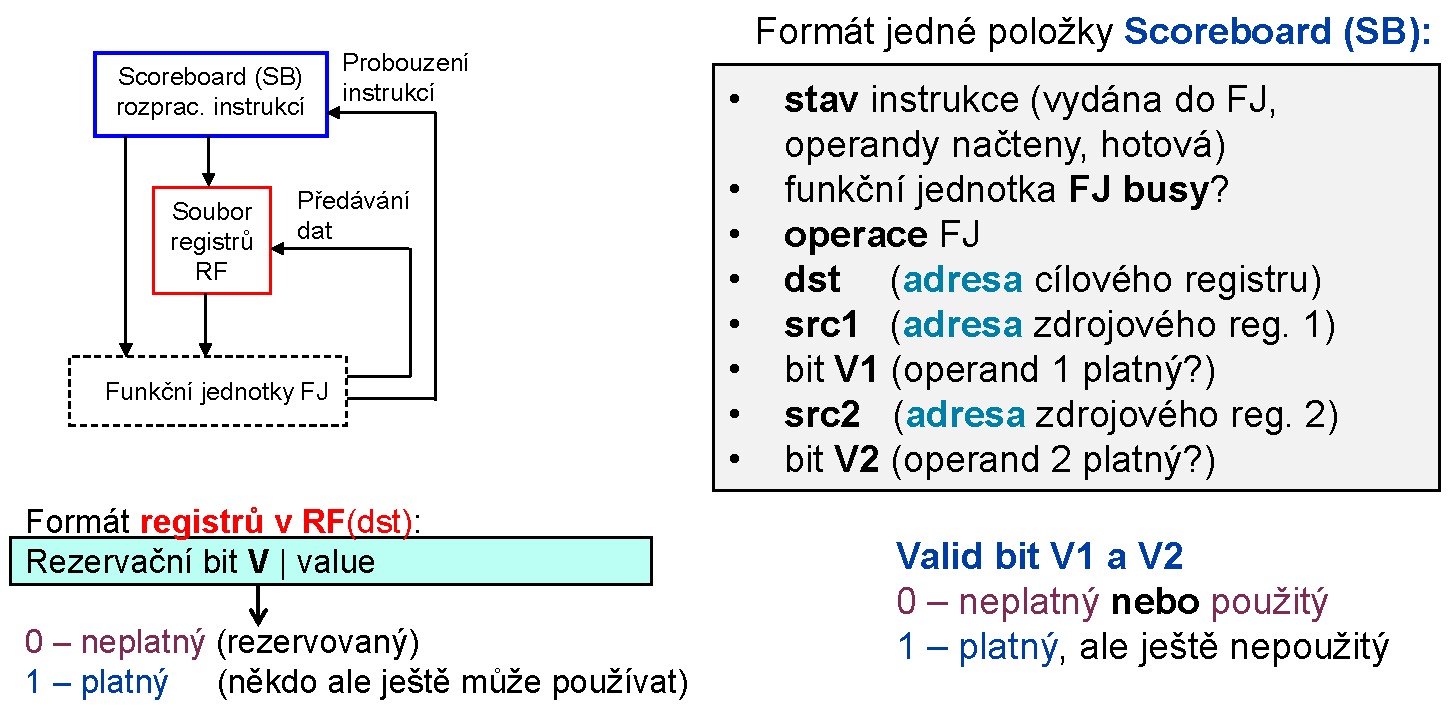
\includegraphics[width=1\linewidth]{score_board.pdf}
        \caption{Princip algoritmu.}
    \end{figure}

    \item Formát: \begin{compactitem}
        \item Registrové pole (\textit{register field}) -- Identifikátor registru, Valid bit, Hodnota.
        \item Tabulka skóre (\textit{score board}) -- Stav instrukce, Funkční jednotka, Operace, DST (adresa), SRC1 (adresa), Valid bit1, SRC2 (adresa), Valid bit2.
    \end{compactitem}

    \item \textbf{Postup algoritmu:} \begin{compactenum}
        \item Rezervace cílového registru v poli registrů (kvůli WAW konfliktu). \begin{compactenum}
            \item Registr má valid bit na 1. Hodnota v něm je platná a žádná instrukce do něho nezapisuje. Můžu nastavit na 0 a tím si registr zarezervovat.

            \item Registr má valid bit na 0. Do registru právě generuje výsledek jiná instrukce, musím čekat.
        \end{compactenum}

        \item Při rezervování cílového registru je přidán daný záznam do tabulky skóre a je vyplněn příslušnými hodnotami z registrového pole (kvůli RAW konfliktu). \begin{compactenum}
            \item Pokud jsou valid bity zdrojových registrů nastaveny na 1, znamená to, že všechny předcházející instrukce, které s nimi pracovali už skončili. Můžu z nich natáhnout data do funkční jednotky a jejich valid bity v tabulce skóre nastavim na 0, aby do registrů mohli zapisovat další instrukce.
            \item Pokud je aspoň jeden valid bit zdrojových registrů na 0, znamená to, že data v nich ještě nejsou aktuální. Jiná instrukce do nich ještě zapisuje a já musím čekat.
        \end{compactenum}

        \item Mám výsledek z funkční jednotky (kvůli WAR konfliktu). \begin{compactenum}
            \item Pokud se v tabulce skóre můj cílový registr vůbec nenachází a nebo se nachází jako zdrojový a má valid bit na 0, tak můžu výsledek zapsat do registrového pole.
            \item Pokud se v tabulce skóre můj cílový registr nachází jako zdrojový a má valid bit na 1, tak jiná instrukce s jeho starou hodnotou ještě bude pracovat a já musím čekat.
        \end{compactenum}

        \item Smažu záznam z tabulky skóre.
    \end{compactenum}

    \begin{figure}[H]
        \centering
        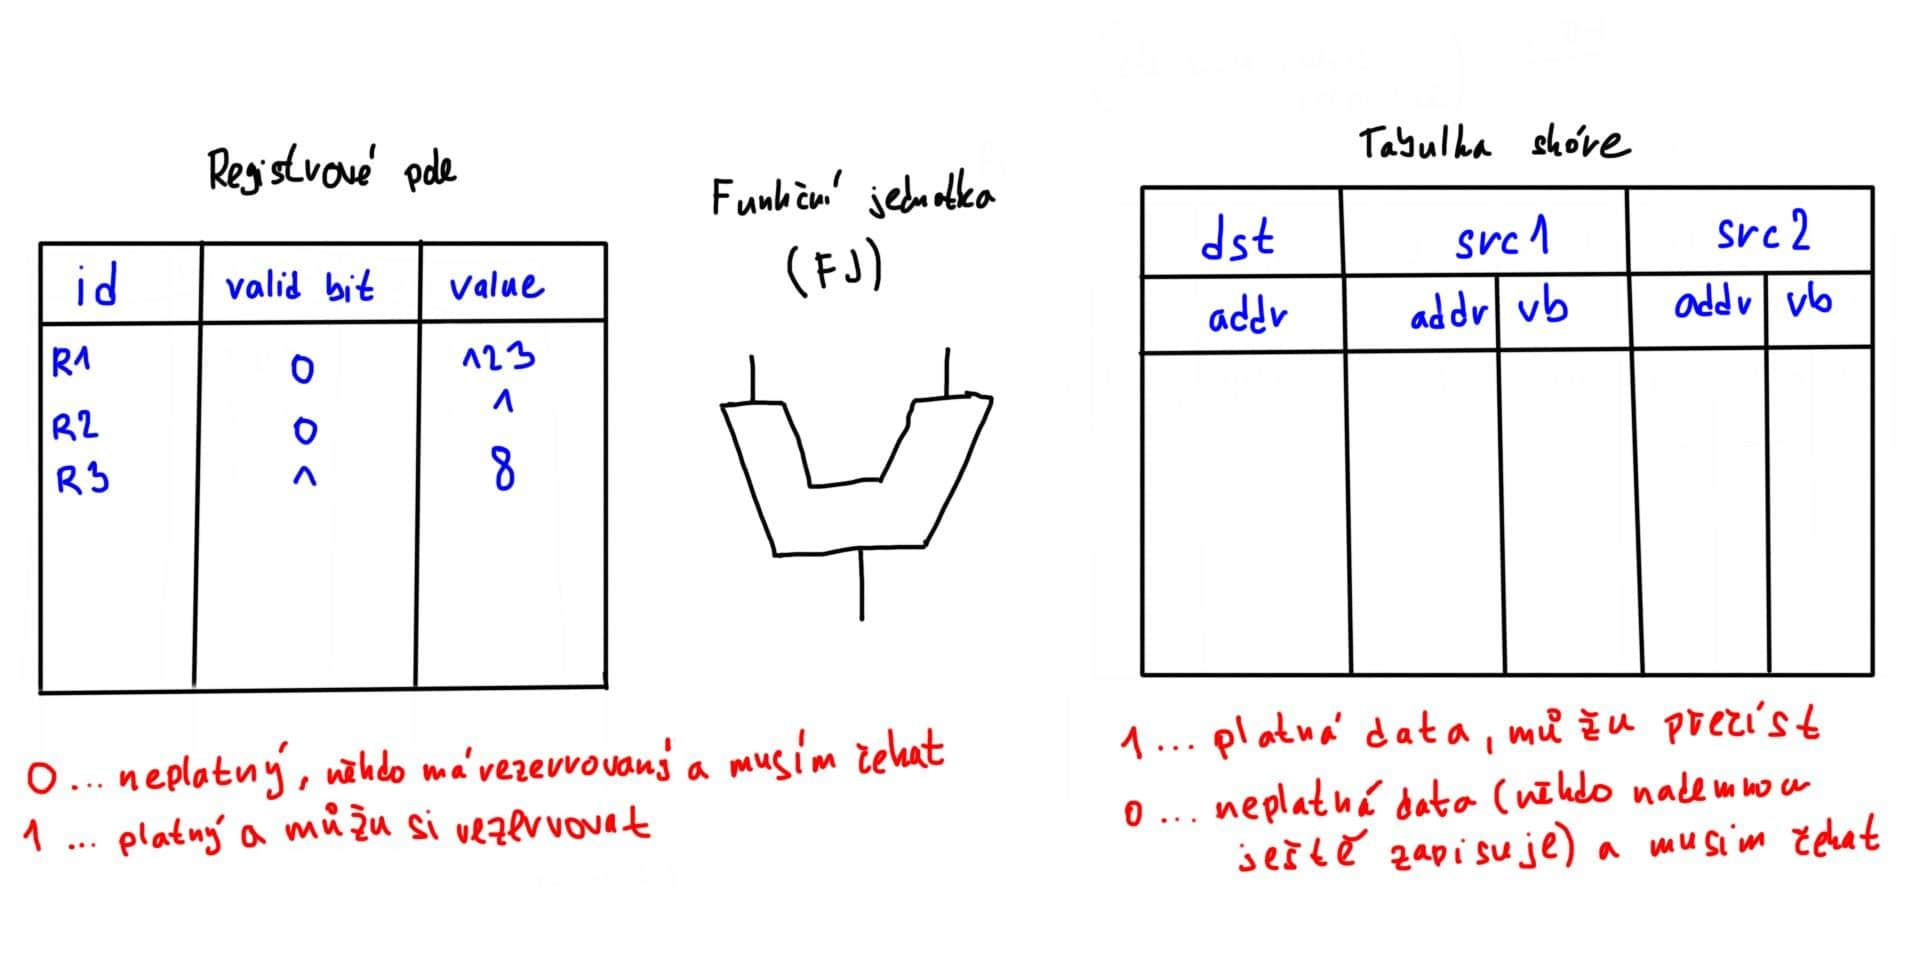
\includegraphics[width=1\linewidth]{example_score_board.jpg}
        \caption{Příklad algoritmu Scoreboarding.}
    \end{figure}
\end{compactitem}

\subsection{Rezervační stanice (Tomasolův algoritmus)}

\begin{compactitem}
    \item Buď individuální nebo společná rezervační stanice, konflikty se řeší přejmenováním, tj. uložením do jiného registru.

    \item Registr může být přejmenován několikrát, ale do původního registru nemusí být uložena každá hodnota, která vznikne prácí s jeho přejmenovanou verzí.

    \item Myšlenka: přejmenovávám cílové registry, tak řeším nepravé konflikty a výsledky ukládám jinám, tj. nečekám.

    \item Shrnutí konfliktů: RAW se řeší čekáním, nelze jinak, ale mezitím můžeme vykonávat jinou instrukci. WAR a WAW se řeší pomocí přejmování a příznaků.

    \item Formát: \begin{compactitem}
        \item Registrové pole (register field): Jméno, Tag, Valid bit, Hodnota.
        \item Rezervační stanice: DST adresa, DST tag, SRC1 valid bit, SRC1 tag, SRC1 hodnota, SRC2 valid bit, SRC2 tag, SRC2 hodnota.
    \end{compactitem}

    \item \textbf{Postup algoritmu:} \begin{compactenum}
        \item Cílovému registru v poli registrů dám nové jméno, tzv. tag, v rezervační stanici vytvořím nový záznam a vyplním DST. \begin{compactenum}
            \item V poli registrů udržuji pouze poslední přejmování.
        \end{compactenum}

        \item Natáhnutí zdrojových registrů do rezervační stanice. \begin{compactenum}
            \item Pokud jsou valid bity zdrojových registrů v poli registrů na 1, vyplním v rezervační stanici celý SRC (valid bit, tag a hodnotu).
            \item Pokud nějaký z valid bitů zdrojových registrů je na 0, vyplním v rezervační stanici valid bit a tag (poslední přejmování), na hodnotu čekám -- dodá mi ji FJ.
        \end{compactenum}

        \item Pokud mají oba zdrojové operandy valid bit na 1, tak je oprace spuštěna a funkční jednotka vypočítá výsledek, který dá na společnou sběrnici (id, tag, value).

        \item Nahrání dat ze společné sběrnice. \begin{compactenum}
            \item Rezervační stanice monitoruje společnou sběrnici. Pokud se nějaký tag shoduje s tagem zdroje v rezervační stanici, který má valid bit na 0, tak si hodnotu vezme valid bit je nastaven na 1.
            \item Registrové pole taktéž monitoruje společnou sbernici. Hledá stejnou dvojici registr id, tag, když najde tak si vezme výsledek. (bere až poslední přejmenování)
        \end{compactenum}
    \end{compactenum}

    \begin{figure}[H]
        \centering
        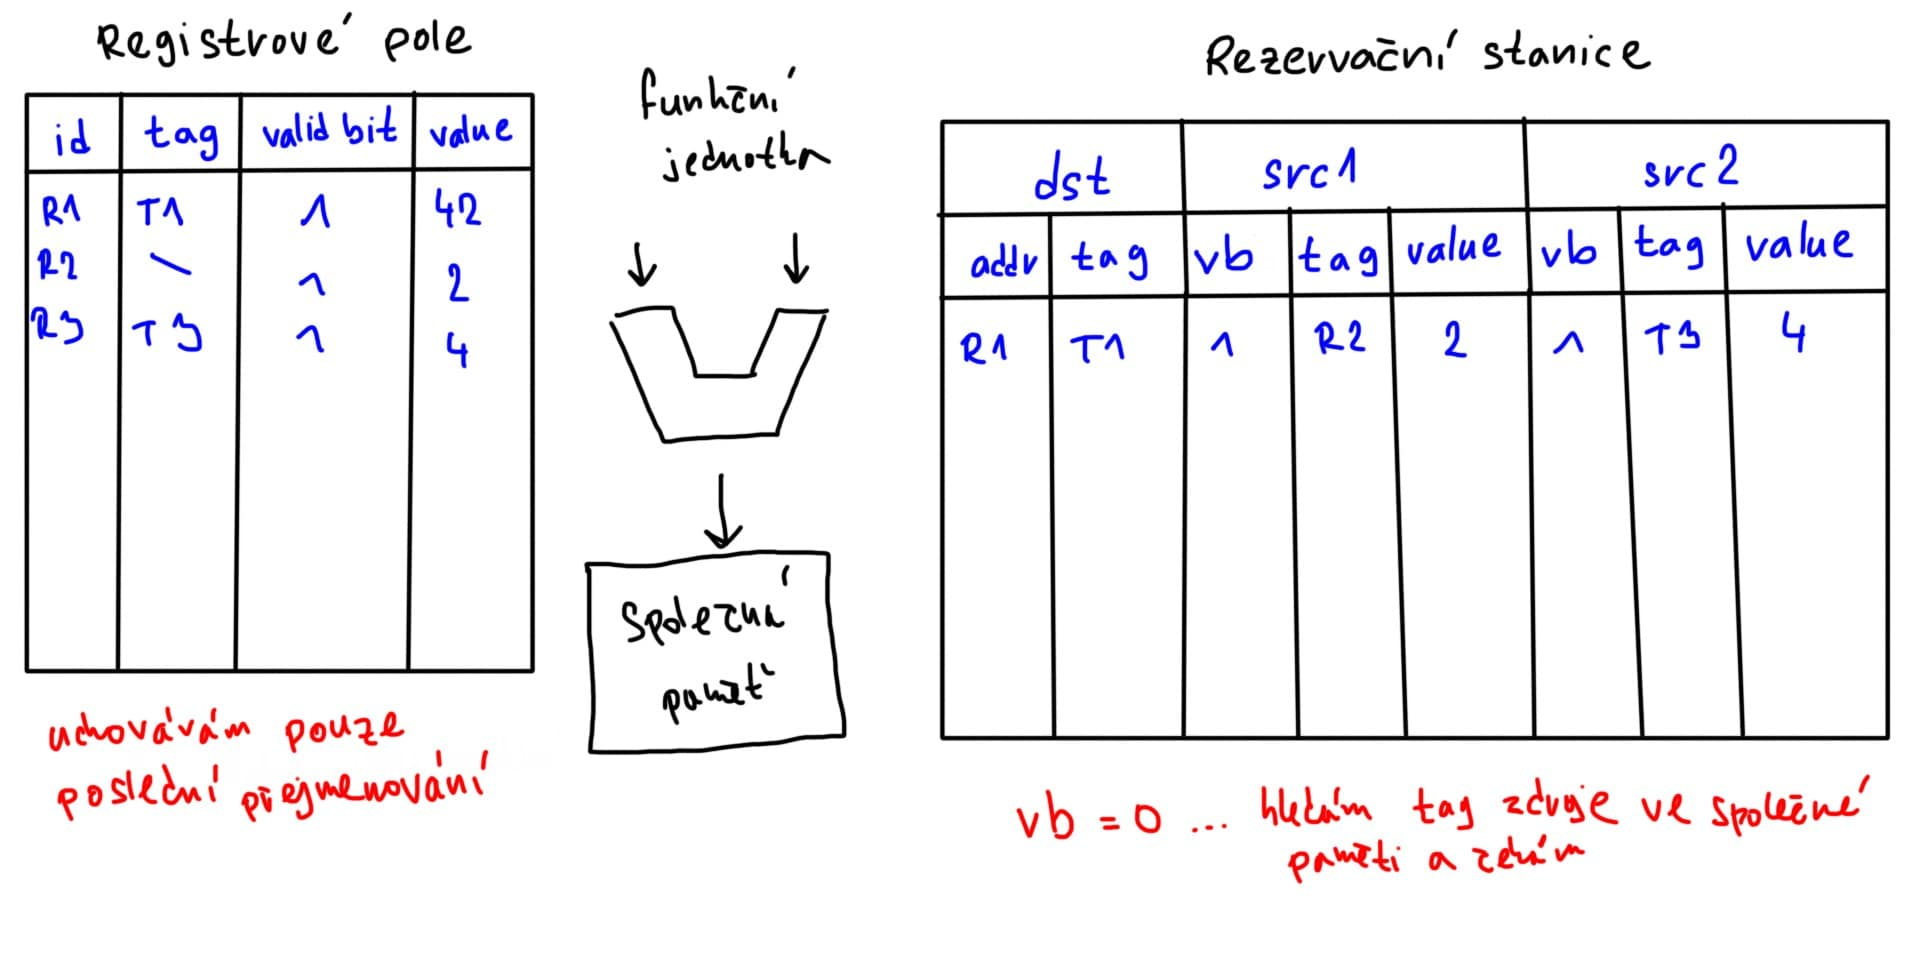
\includegraphics[width=1\linewidth]{example_reserve_stations.jpg}
        \caption{Příklad algoritmu Rezervační stanice.}
    \end{figure}
\end{compactitem}

%%%%%%%%%%%%%%%%%%%%%%%%%%%%%%%%%%%%%%%%%%%%%%%%%%%%%%%%%%%%%%%%%%%%%%%%%%%%%%%%

\section{Predikce skoků}

\begin{compactitem}
    \item Pro superskalární procesor čekat 1 takt při skoku je špatné, jsou třeba prediktory skoku a čekání kompletně eliminovat.

    \item Skoky jsou vysoce předvídatelné, můžeme je predikovat.

    \item Prediktor se nachází hned ve fázi IF. \begin{compactitem}
        \item Pamatuje si, kam se v minulosti skákalo (má uložené adresy).
        \item Pokud ji najde, ví že se jedná o skok
    \end{compactitem}

    \item Pokud narazíme na skokovou instrukci, tak spekulujeme, ale nikdy si nejsme jistí. K instrukci je přidám příznak (spekulativní bit), který je později v případě korektní spekulace odstraněn, případně ponechám a příznaky se použijí k odstranění těchto instrukcí z ROB (\textit{re-order buffer}) a RS (rezervační stanice).

    \begin{figure}[H]
        \centering
        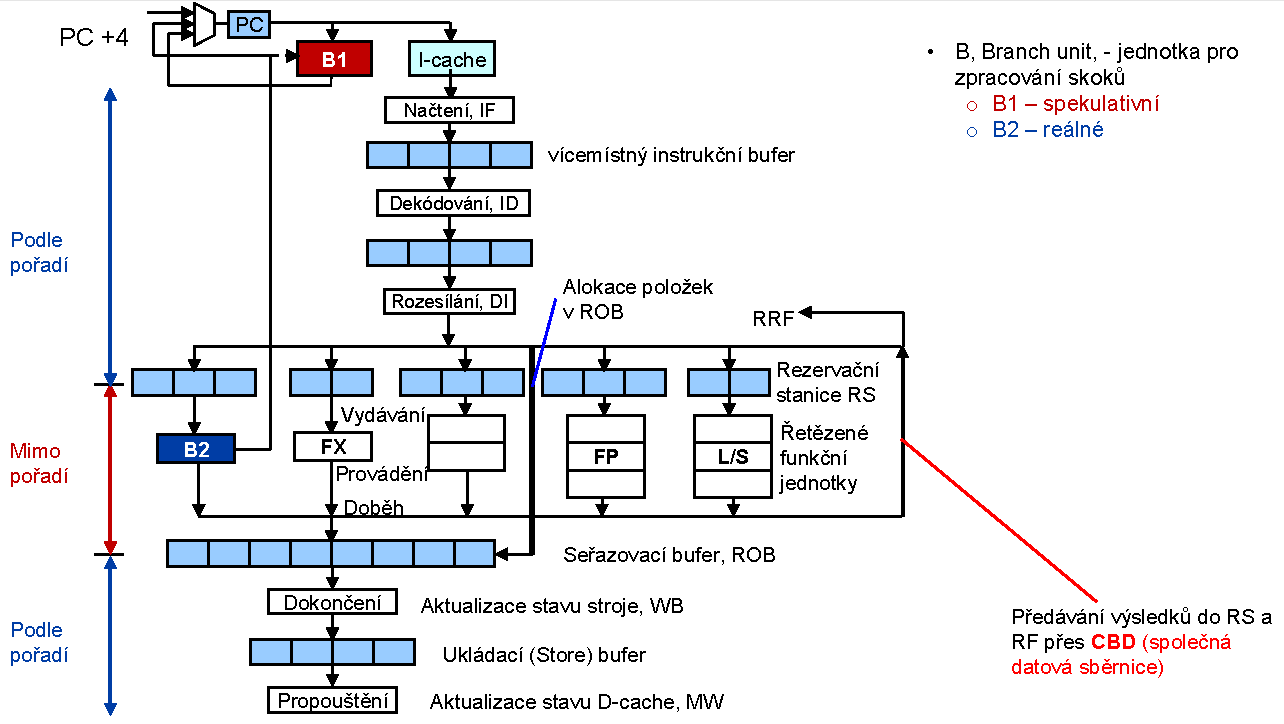
\includegraphics[width=1\linewidth]{umisteni_prediktoru.pdf}
        \caption{Umístění prediktoru skoků.}
    \end{figure}
\end{compactitem}

\subsection{Predikce podmínky skoku}

\begin{compactitem}
    \item Predikujeme, jestli se bude skákat, nebo nikoliv (týká se pouze podmíněných skoků).
\end{compactitem}

\subsubsection{1-bitový prediktor}

\begin{compactitem}
    \item Tabulka BHT (\textit{branch history table}), která obsahuje adresu instrukce a u toho informaci, jestli se z ní posledně skákalo (1 bit). \begin{compactitem}
        \item 0 -- spekuluju, že se nebude skákat.
        \item 1 -- spekuluju, že se bude skákat.
    \end{compactitem}
    \item Hned po IF můžu porovnavat.
    \item Pokud narazím na novou instrukci skoku, zjistim to až v ID, přidám ji do tabulky a po fázi EX k ní vložím / aktualizuji záznam, jestli jsem skočil.

    \begin{figure}[H]
        \centering
        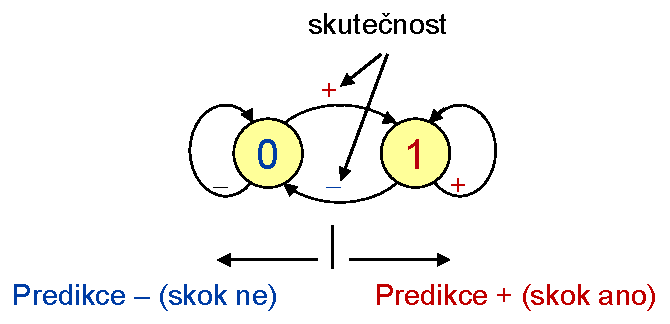
\includegraphics[width=0.5\linewidth]{prediktor_jednobitovy.pdf}
        \caption{1-bitový prediktor.}
    \end{figure}
\end{compactitem}

\subsubsection{2-bitový prediktor}

\begin{compactitem}
    \item Stejný princip, pouze máme 2 bity.
    \item Vyšší bit říká, jestli máme skočit: \begin{compactitem}
        \item 00, 01 -- spekuluju, že se nebude skákat.
        \item 10, 11 -- spekuluju, že se bude skákat.
    \end{compactitem}
    \item Je schopen velice dobře rozeznat vnořené smyčky

    \begin{figure}[H]
        \centering
        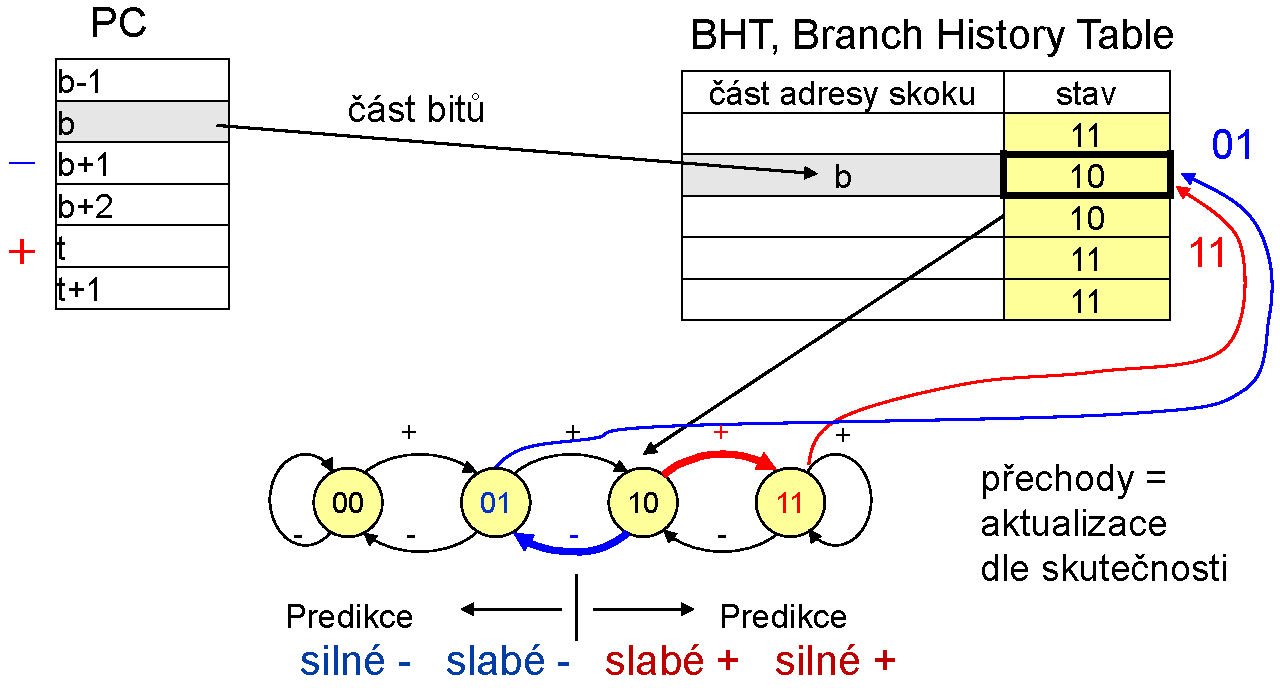
\includegraphics[width=0.75\linewidth]{prediktor_dvoubitovy.pdf}
        \caption{2-bitový prediktor. Příklad: adresu b jsem našel v tabulce, tj. je to skoková instrukce. Je ve stavu 10, tedy budu spekuluji, že budu skákat. Později se dozvím, že jsem skočil správně, přejdu do stavu 11 a vše je v pořádku. Nebo se dozvím, že jsem se spletl a skákat jsem neměl, přejdu do stavu 01 a je třeba větev výpočtu zahodit.}
    \end{figure}
\end{compactitem}

\subsubsection{Adaptivní prediktor s lokálními BHSR (\textit{branch history shift register})}

\begin{compactitem}
    \item Stejný jako 2-bitový prediktor, pouze mám k dispozici několik dvoubitových prediktorů a posuvný registr.
    \item Posuvný registr mi říká, který prediktor použít, na základě historie skoků, které si pamatuje.
    \item Je se schopný naučit nějaké vzorce chování, čím větší posuvný registr, tím složitější patterny.
    \item Konkrétněji: \begin{compactitem}
        \item Máme 4 čítače, každá má jiný výchozí stav
        \item Všechny se aktualizují vždy
        \item Podle historie vybírám ten, který se mi nejvíc hodí
    \end{compactitem}

    \begin{figure}[H]
        \centering
        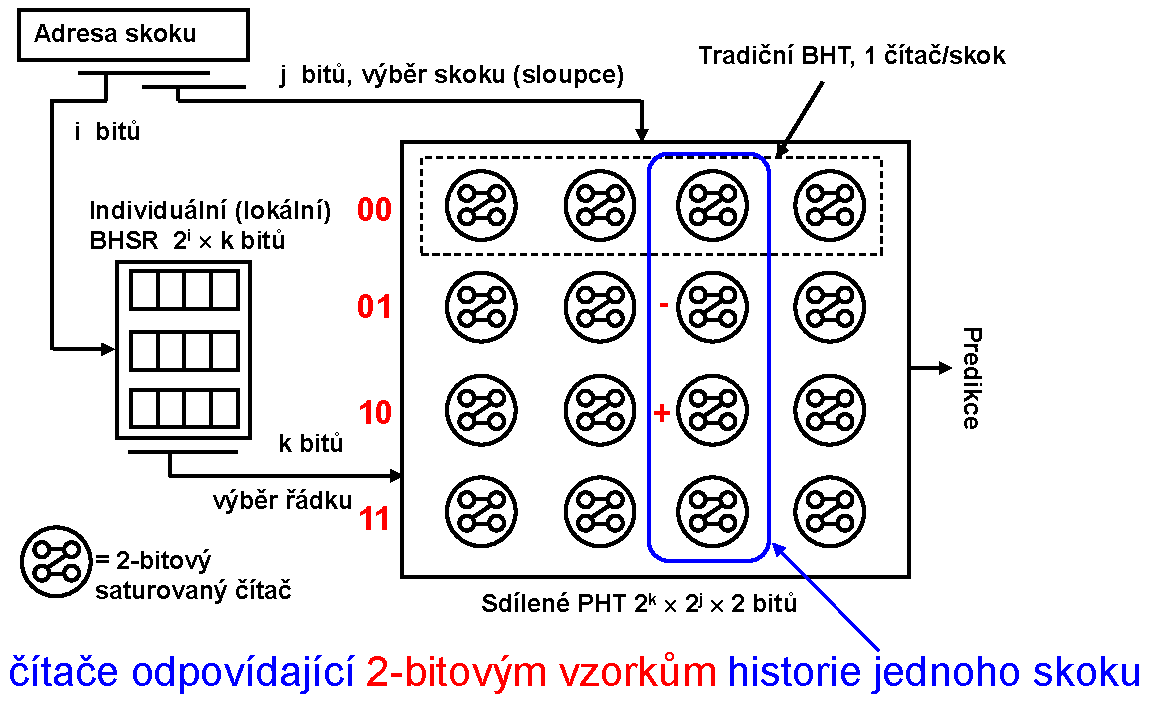
\includegraphics[width=0.85\linewidth]{prediktor_adaptivni.pdf}
        \caption{Adaptivní prediktor s lokálními BHSR.}
    \end{figure}
\end{compactitem}

\subsection{Predikce cílovej adresy}

\begin{compactitem}
    \item Predikujeme, kam se bude skákat.
    \item Tabulka kde je uložené na jaké adresy se skákalo.
    \item Intuice: \begin{compactitem}
        \item Když prediktor podmínky skokové instrukce (BHT) říká \uv{bude se skákat}: \begin{compactitem}
            \item a prediktor cílové adresy zná adresu -- skočí se,
            \item a prediktor cílové adresy nezná adresu -- neskočí se.
        \end{compactitem}
        \item Když prediktor podmínky skokové instrukce (BHT) říká \uv{nebude se skákat}, tak se skákat nebude ať má přediktor cílové adresy cokoliv. Prediktor skokové instrukce má vyšší prioritu.
    \end{compactitem}
\end{compactitem}

\subsubsection{Branch Target Address Cache (BTAC)}

\begin{compactitem}
    \item Tabulka, která obsahuje adresu instrukce a informaci jestli se skočilo a kam se skočilo.
\end{compactitem}

\subsubsection{Return Stack Buffer}

\begin{compactitem}
    \item Zásobník návratových adres.
    \item Pro instrukce return.
\end{compactitem}

\begin{figure}[H]
    \centering
    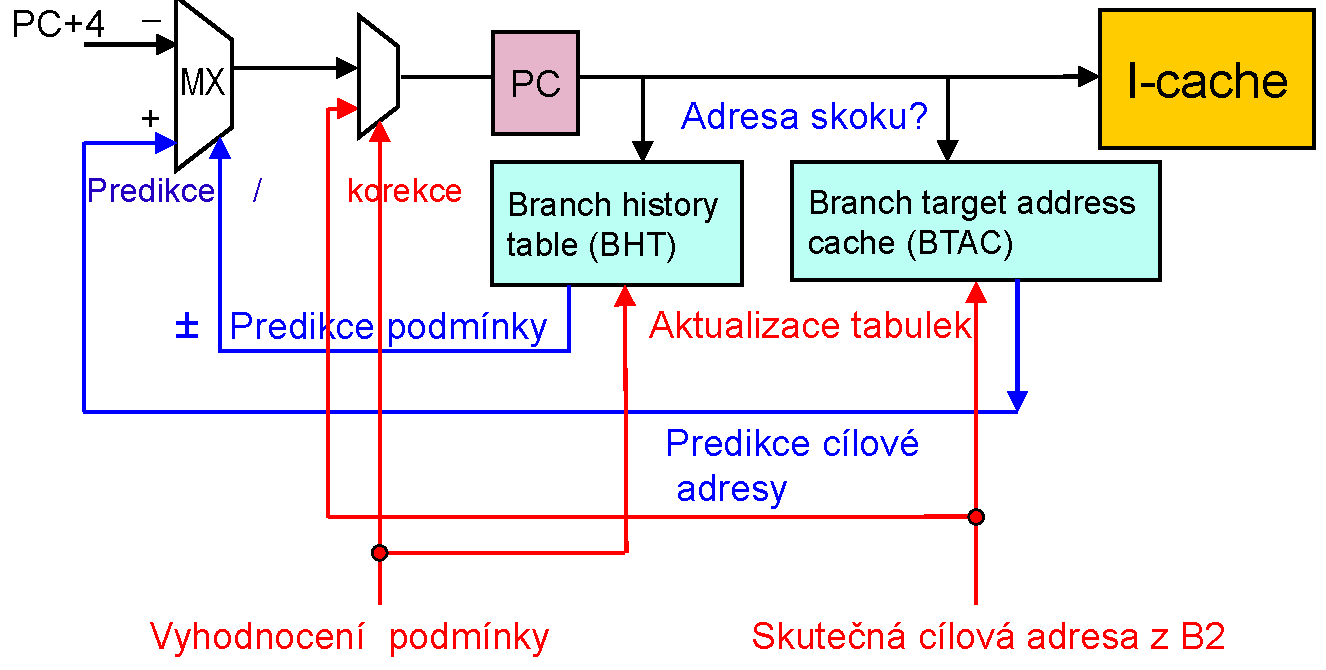
\includegraphics[width=0.8\linewidth]{predikce_podminky_a_cilove_adresy.pdf}
    \caption{Predikce podmínky a cílové adresy.}
\end{figure}
